\documentclass[a4paper,12pt]{beamer}

\usepackage[T3,OT2,T1]{fontenc}
\usepackage[utf8]{inputenc}

\usepackage[british]{babel}

% % latin modern font (disabled because it breaks tipa...)
% \usepackage{lmodern}

\usepackage[normalem]{ulem}

\usepackage{hologo}

\usepackage{tikz}
\usetikzlibrary{arrows.meta}

% Beamer theme
%\usecolortheme{dove}
%\usecolortheme{crane}
%\usecolortheme{orchid}
%\usecolortheme{focus}
\usecolortheme{orchid}
\useinnertheme{circles}
\useoutertheme{infolines}
% disable top bar
\setbeamertemplate{headline}[default]
\usefonttheme{structurebold}

\title{Introduction to \LaTeX}
\author[Johannes Englisch]{%
  Johannes Englisch\\{}%
  \href{mailto:johannes_englisch@eva.mpg.de}{\emph{\footnotesize{}johannes\_englisch@eva.mpg.de}}%
}
% TODO Name of the event.
\date[2\,Oct 2022]{2\,Oct 2022}
\institute[MPI EVA:\ DLCE]{%
  Department of Cultural and Linguistic Evolution\\%
  Max Planck Institute for Evolutionary Anthropology\\%
  Leipzig, Germany%
}

\hypersetup{%
  pdfauthor=Johannes Englisch,%
  pdftitle=Introduction to LaTeX,%
  breaklinks,%
  colorlinks,%
  allcolors=.,%
  urlcolor=blue,%
}

% needs to be loaded as late as possible
\usepackage{gb4e}
% gb4e sets glosses in a serif font by default
\let\eachwordone=\sf%
\let\eachwordtwo=\sf%
\let\eachwordthree=\sf%

% needs to be loaded after gb4e...
\usepackage[noenc]{tipa}


\begin{document}

\maketitle%

\section{Introduction}

\begin{frame}
  \frametitle{Why \LaTeX{}?}

  \begin{block}{Single-slide elevator pitch}
    \begin{itemize}
      \item It makes \alert{beautiful} documents by default.\pause{}
      \item It \alert{automates} a~lot of the tedious busywork (table of
        contents, numbered sections, cross-references, etc.).\pause{}
      \item It's \alert{versatile} (I~made these slides with \LaTeX).\pause{}
      \item The document is saved as \alert{plain text}, which lends itself
        well to version control systems such as \alert{git}.\pause{}
      \item The output is a~PDF, so it looks the same everywhere.
    \end{itemize}
  \end{block}
\end{frame}

\begin{frame}
  \frametitle{Why \LaTeX{}? (ctd.)}

  \begin{block}{Cool stuff out of the box}
    Behold this formula:

    \[%
      f = \lambda x \lambda Y.
      \frac{1}{2}
      \left(%
        \frac{%
          \sqrt[3000]{%
            \frac
            {4 + \frac{x}{12}}
            {\sum_{i=1}^k{y_i}}
          }
          + e^\pi
        }{%
          \tau \sin (x^2 + 0.5x + \epsilon)
        }
      \right)
    \]
  \end{block}

\end{frame}

\begin{frame}
  \frametitle{Why \LaTeX{}? (ctd.)}

  \begin{block}{Third-party packages}
    \LaTeX{} also comes with a~massive collection of third-party packages for
    specific use cases (like numbered examples or glosses).

    \begin{exe}
      \ex%
      \begin{xlist}
        \ex[]{Look, an example!}
        \ex[*]{\label{ex:ungrammatical}Look, an second example!}
      \end{xlist}
      \ex%
      \glll Das ist ein wunderschönes Beispiel! \\
      \textipa{\r*d2s} \textipa{PIs} \textipa{PE} \textipa{"V\|)Un\r*d\|)O\super{Q}""S\t*{eI}n@s} \textipa{"\r*b\t{\ae{}I}S\r*bi:l} \\
      this is a beautiful example \\
      \glt `This is a~beautiful example!'
    \end{exe}

    \emph{\footnotesize%
      (Look how nicely the star in~(\ref{ex:ungrammatical}) lines up!)
    }
  \end{block}
\end{frame}

\begin{frame}
  \frametitle{Nothing is ever perfect}

  \begin{block}{Downsides}
    \begin{itemize}
      \item Not really suitable for tasks that require finegrained control over
        the graphical design (the slides are already pushing it).
      \item \LaTeX{}'s error messages can be a~bit\dots\ opaque at times.
      \item Passing \LaTeX{} documents around across different computers can
        sometimes be a~bit janky.
      \item Documents that contain multiple languages/scripts is not as
        straight-forward as it could be
        (\hologo{XeLaTeX} tries to address this).
    \end{itemize}
  \end{block}
\end{frame}

\section{What is \LaTeX{}?}

\begin{frame}
  \frametitle{Little history lesson}

  \begin{block}{\TeX}
    \begin{itemize}
      \item Pronounced \textipa{[tEk]}
        {\footnotesize{}(or \textipa{[tEx]}, \textipa{[tE\c{c}]}, etc.)}
      \item Created in 1978 by Donald Knuth.
      \item Computerised type-setting system.
      \item Nowadays considered a~bit too low-level for day-to-day use.
    \end{itemize}
  \end{block}

  \pause{}

  \begin{block}{\LaTeX}
    \begin{itemize}
      \item Pronounced \textipa{[lA:tEk]} or \textipa{[leItEk]}.
        {\footnotesize{}(or \textipa{[-tEx]}, \textipa{[-tE\c{c}]}, etc.)}
      \item Created in 1984 by Leslie Lamport.
      \item Built on top of \TeX.
      \item Provides a~way smoother experience when making documents.
    \end{itemize}
  \end{block}
\end{frame}

\section{How a~\LaTeX{} document comes to be}

\begin{frame}
  \frametitle{WYSIWYG vs.\ WYSIWYM}
  % XXX: possibly move this after the type-setting metaphor

  \begin{block}{`What You See Is What You Get'}
    \begin{center}
      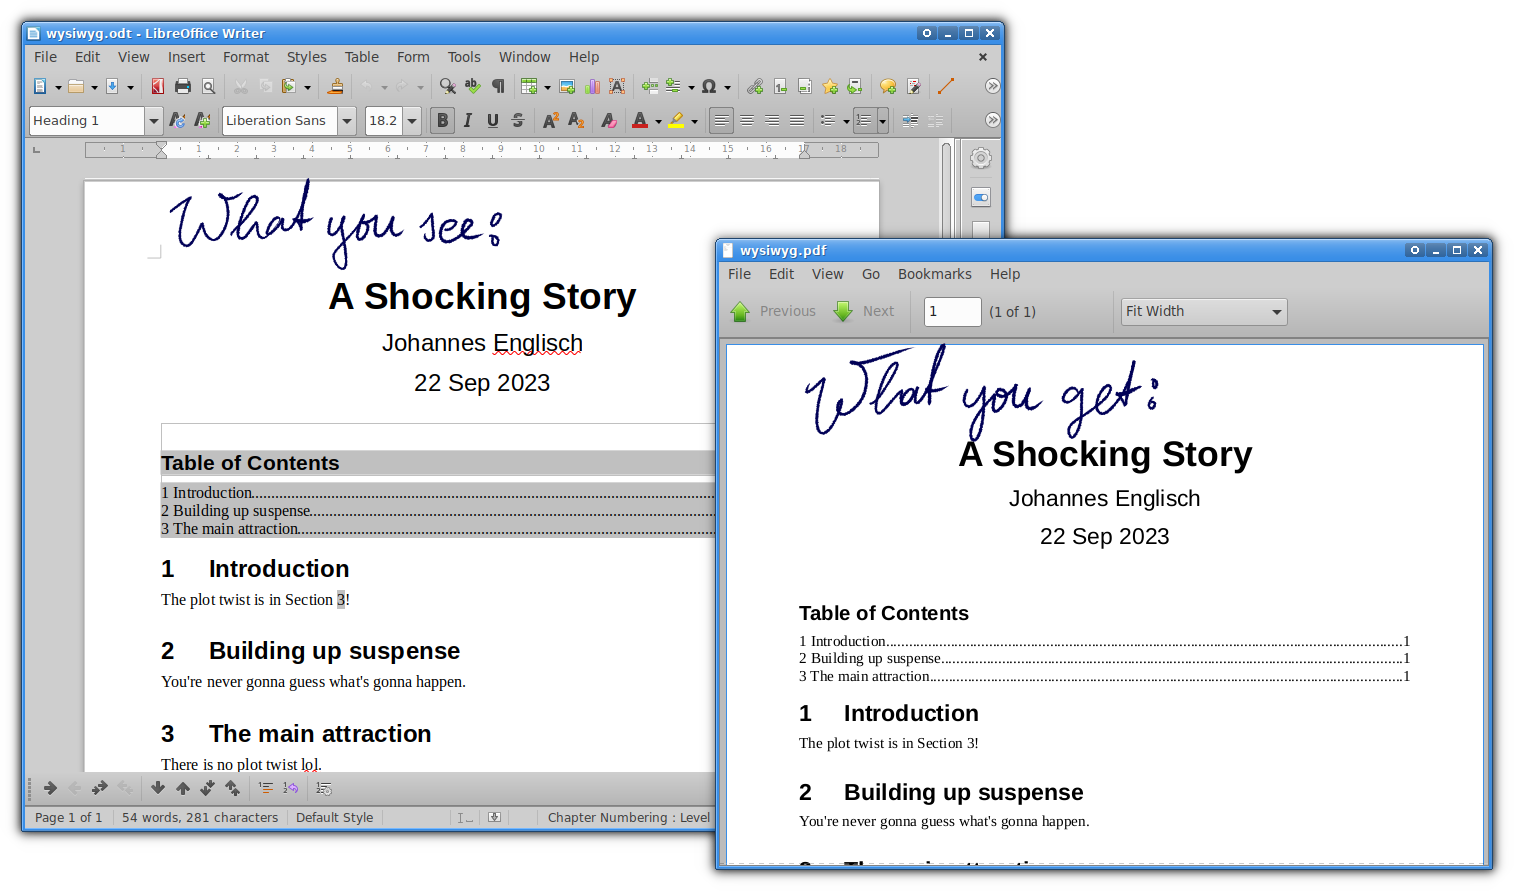
\includegraphics[width=0.85\textwidth]{images/wysiwyg.png}
    \end{center}
  \end{block}
\end{frame}

\begin{frame}
  \frametitle{WYSIWYG vs.\ WYSIWYM (ctd.)}

  \begin{block}{`What You See Is What You \emph{Mean}'}
    \begin{center}
      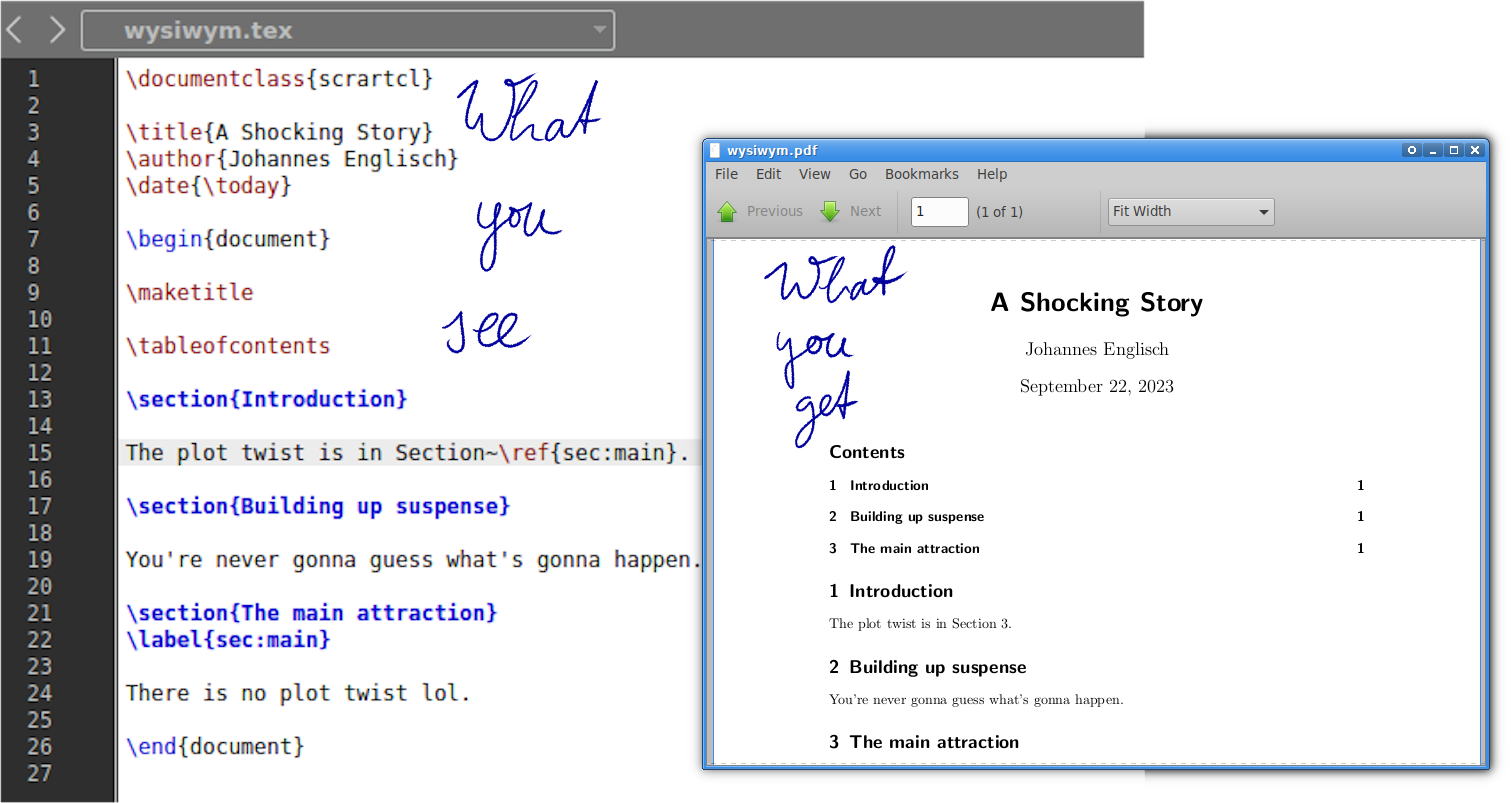
\includegraphics[width=0.85\textwidth]{images/wysiwym.png}
    \end{center}
  \end{block}
\end{frame}

\begin{frame}
  \frametitle{How it works}

  \begin{center}
    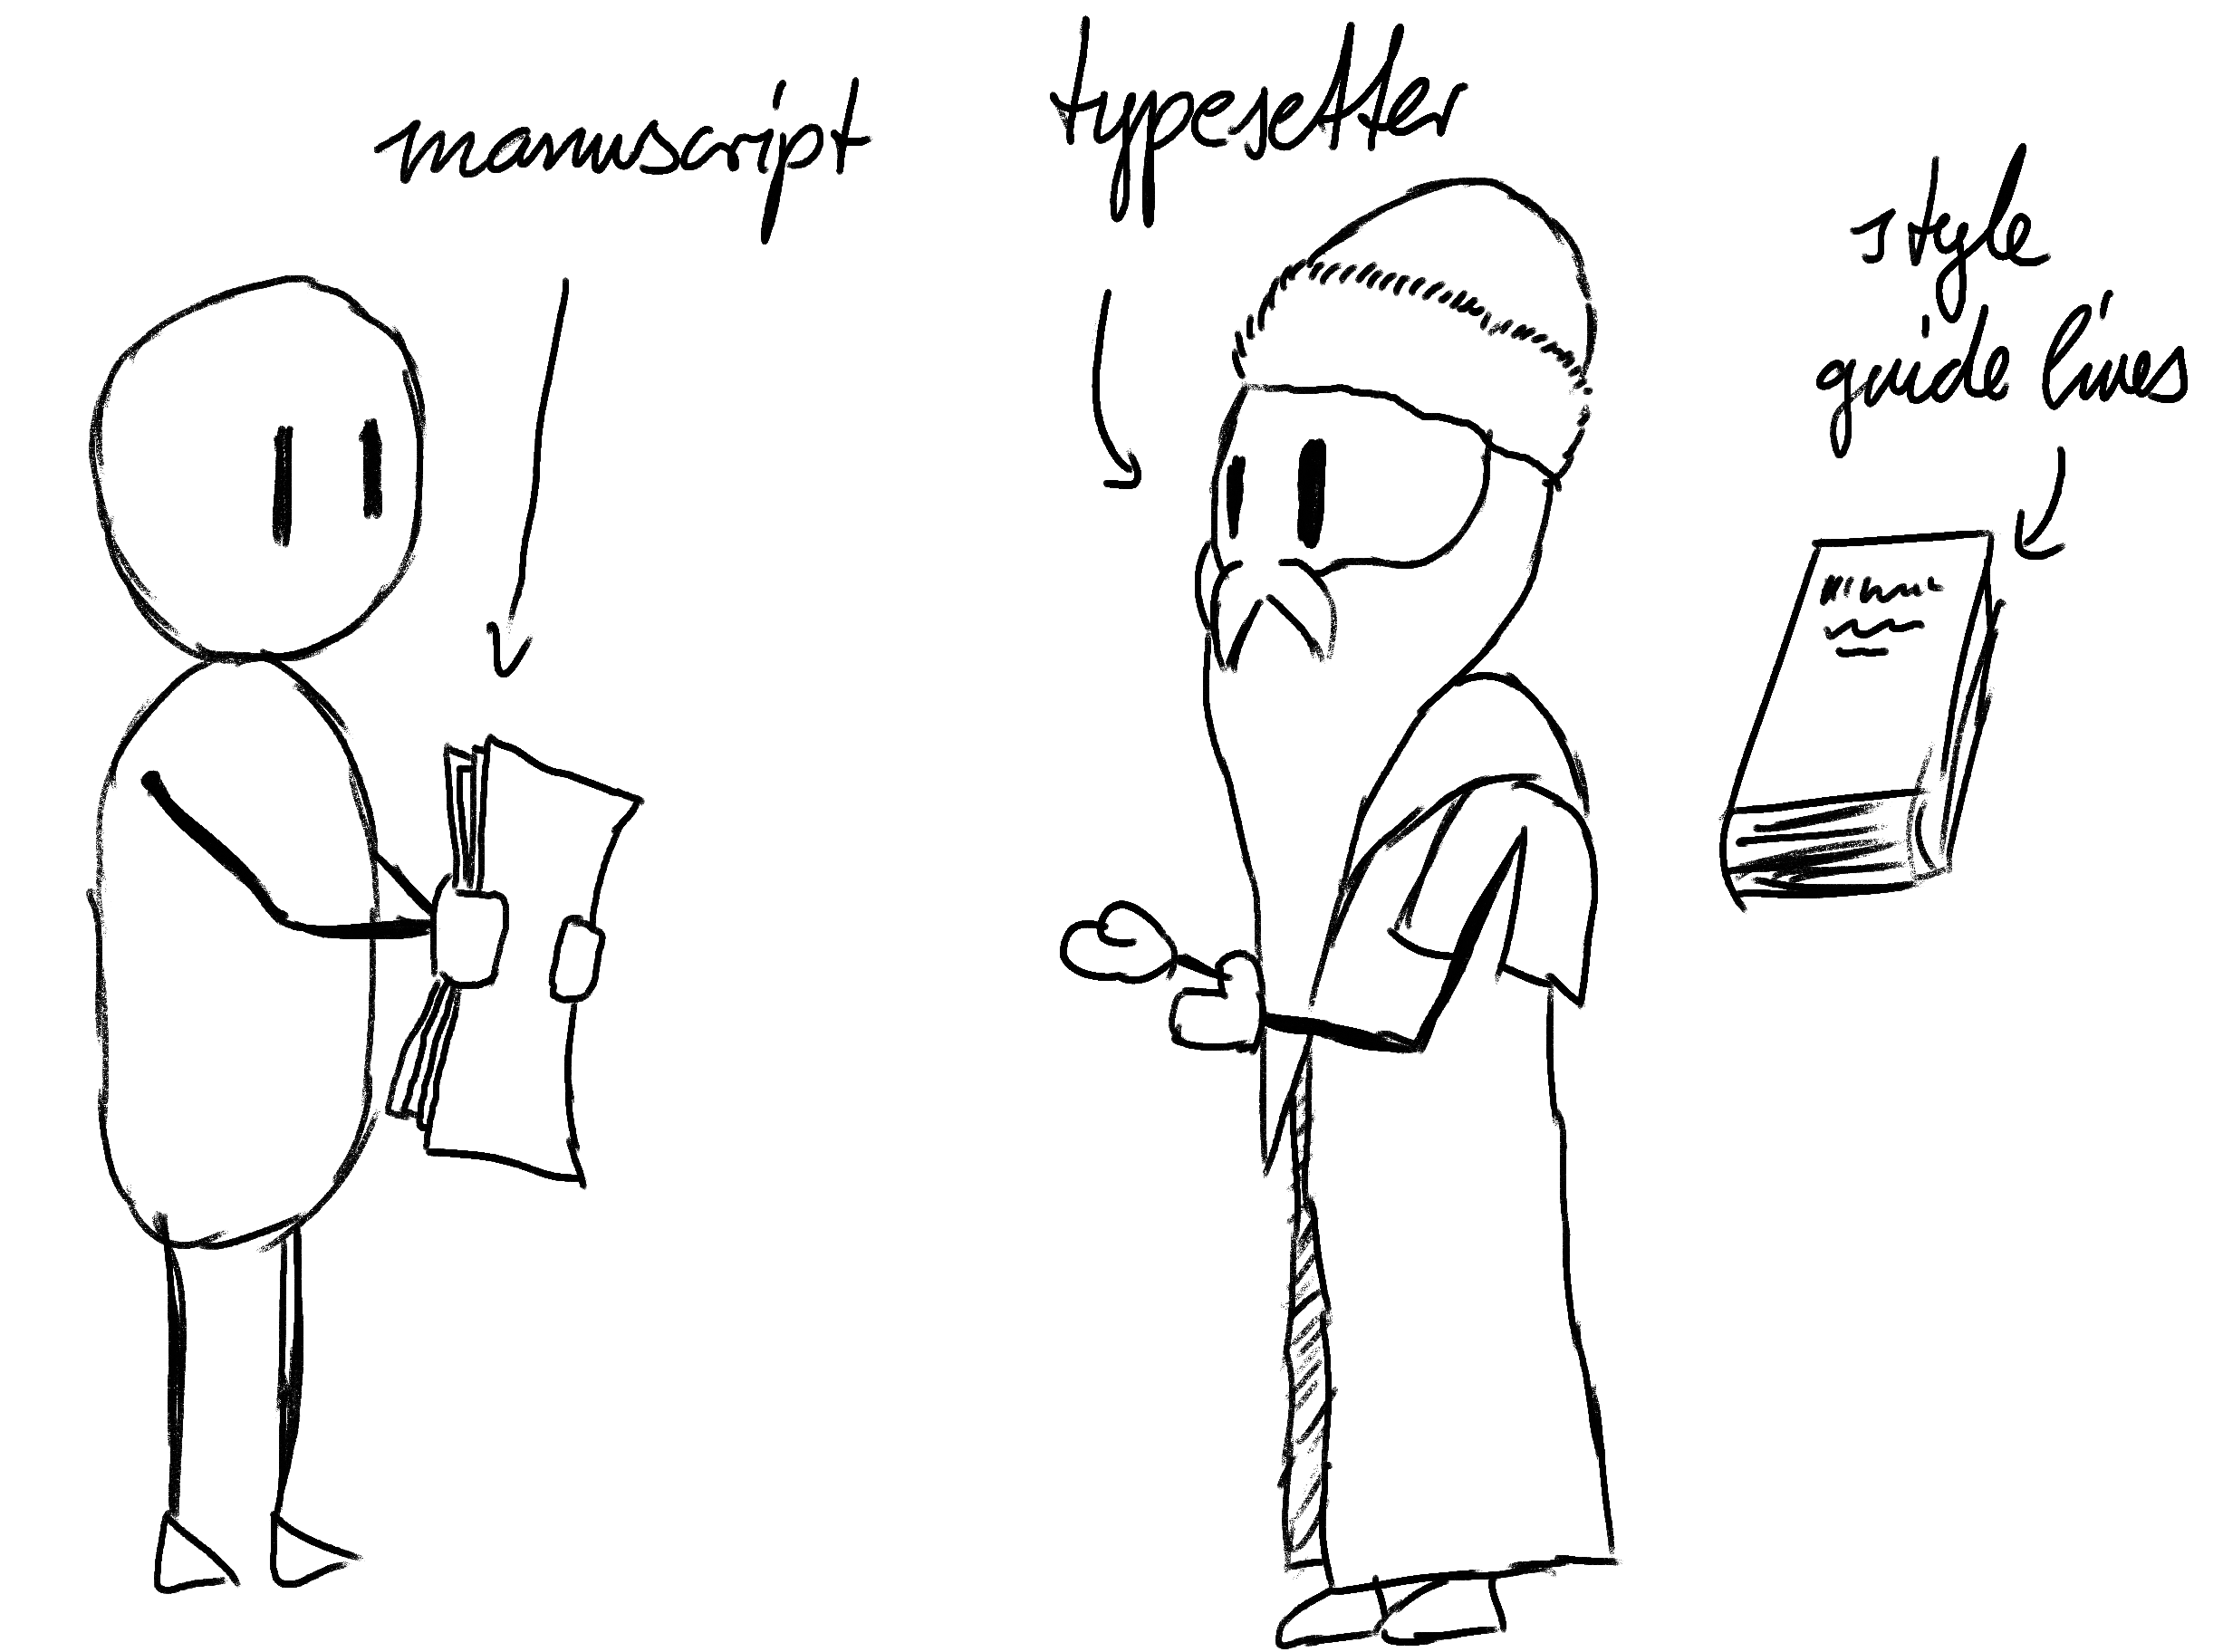
\includegraphics[width=0.75\textwidth]{images/typesetting-then.png}\\
    Type-setting then
  \end{center}
\end{frame}

\begin{frame}
  \frametitle{How it works (ctd.)}

  \begin{center}
    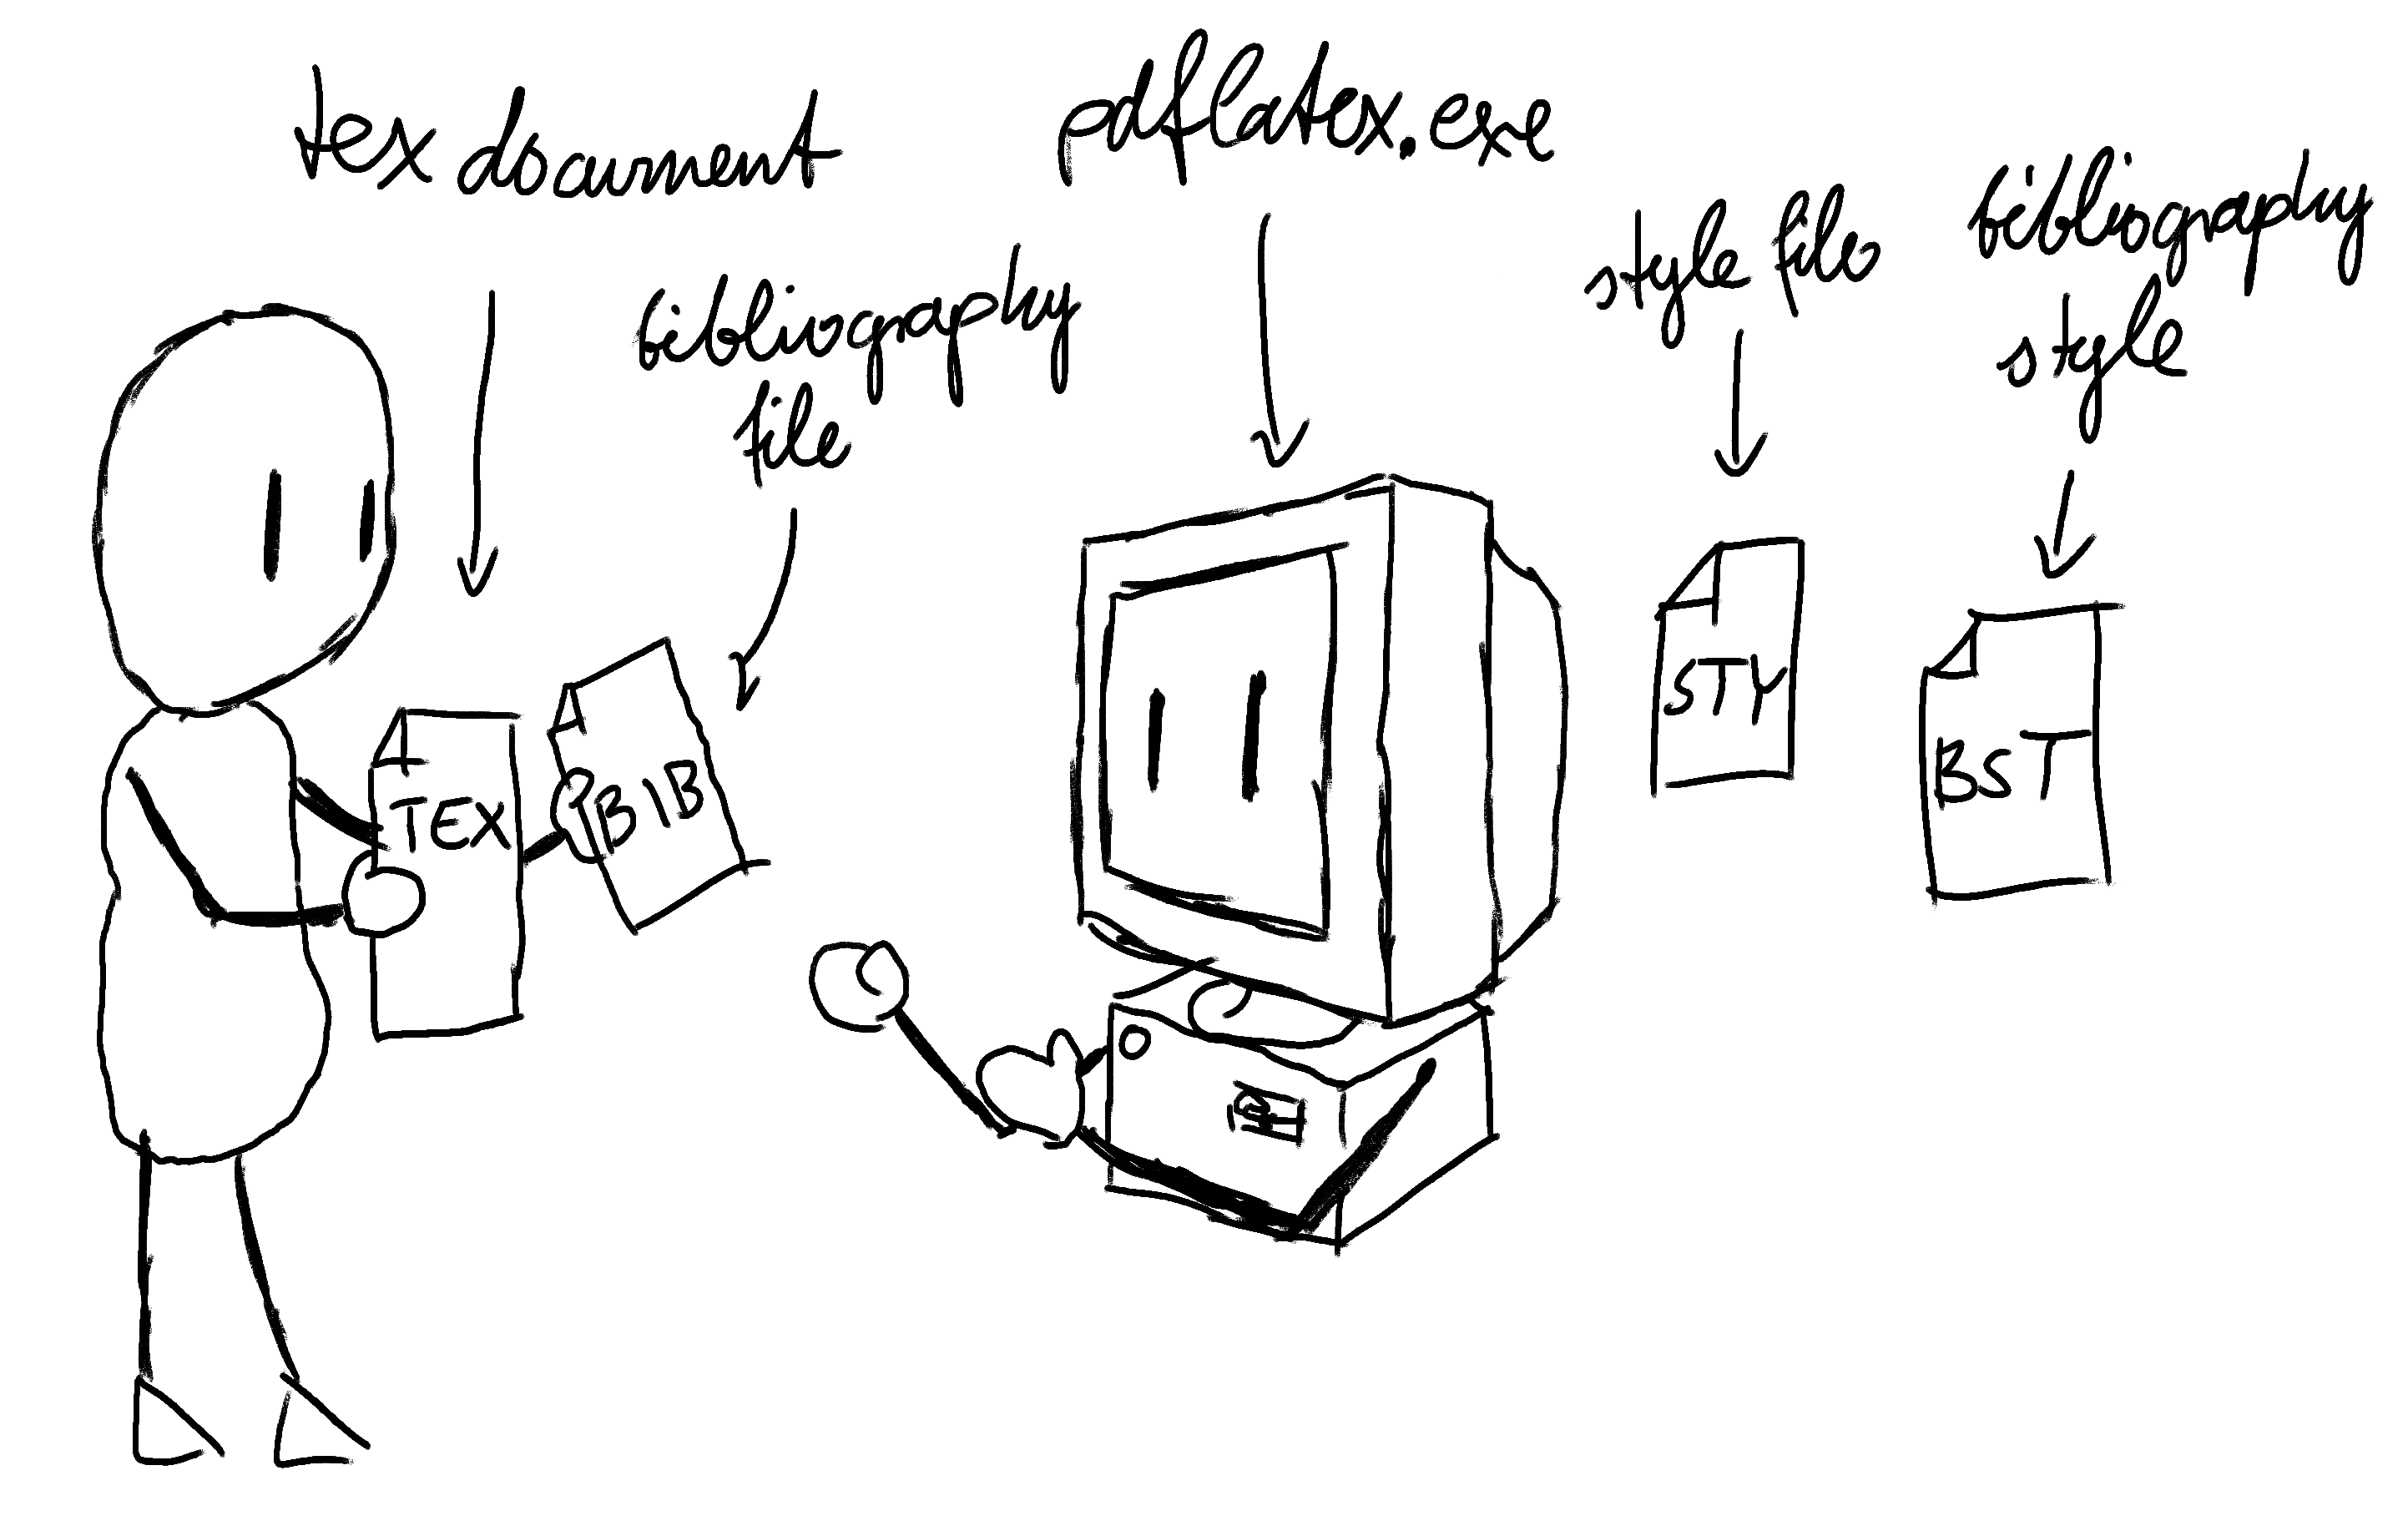
\includegraphics[width=0.75\textwidth]{images/typesetting-now.png}\\
    Type-setting now
  \end{center}
\end{frame}

\begin{frame}
  \frametitle{Where do the files come from?}
  
  \begin{block}{The manuscript}
    \begin{itemize}
      \item \emph{The \TeX{} file:}\ Written by you.
      \item \emph{The \hologo{BibTeX} file:}\ Can be hand-written; in practice
        people export them from their favourite bibliography program.
    \end{itemize}
  \end{block}
  
  \begin{block}{The style guide}
    \begin{itemize}
      \item \emph{The style file:}\ Either from your \LaTeX{} installation or
        provided by publisher/journal.
      \item \emph{The bibliography style:}\ Provided by publisher/journal;
        there's also a~script you can use to make your own.
    \end{itemize}
  \end{block}
\end{frame}

\begin{frame}
  \frametitle{How the \xout{sausage} PDF is made}

  \begin{center}
    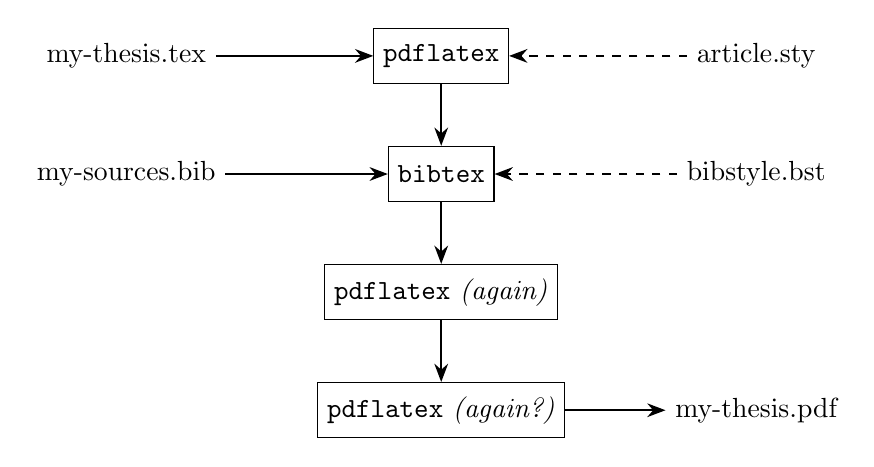
\begin{tikzpicture}
      [program/.style={rectangle,draw,minimum height=2em},>=Stealth]
      \node[program] (pdflatex1) at (0, 0) {\texttt{pdflatex}} ;
      \node[program] (bibtex) at (0, -1.5) {\texttt{bibtex}} ;
      \node[program] (pdflatex2) at (0, -3) {\texttt{pdflatex} \emph{(again)}} ;
      \node[program] (pdflatex3) at (0, -4.5) {\texttt{pdflatex} \emph{(again?)}} ;
      \node (texdoc) at (-4, 0) {my-thesis.tex} ;
      \node (texsty) at (4, 0) {article.sty} ;
      \node (bibdoc) at (-4, -1.5) {my-sources.bib} ;
      \node (bibsty) at (4, -1.5) {bibstyle.bst} ;
      \node (pdfdoc) at (4, -4.5) {my-thesis.pdf} ;
      \draw[->,thick] (pdflatex1) to (bibtex) ;
      \draw[->,thick] (bibtex) to (pdflatex2) ;
      \draw[->,thick] (pdflatex2) to (pdflatex3) ;
      \draw[->,thick] (texdoc) to (pdflatex1) ;
      \draw[->,thick,dashed] (texsty) to (pdflatex1) ;
      \draw[->,thick] (bibdoc) to (bibtex) ;
      \draw[->,thick,dashed] (bibsty) to (bibtex) ;
      \draw[->,thick] (pdflatex3) to (pdfdoc) ;
    \end{tikzpicture}
  \end{center}
  \emph{\footnotesize{}(No worries, you don't have to do this manually.)}
\end{frame}

\begin{frame}
  \frametitle{What do you need?}

  \begin{block}{\LaTeX{} itself}
    \begin{itemize}
      \item Windows:\ \href{https://miktex.org/}{\hologo{MiKTeX}}
      \item macOS:\ \href{https://www.tug.org/mactex/}{Mac\TeX}
        (\href{https://dunglas.dev/2021/09/installing-a-latex-environment-on-a-mac/}{via homebrew}
        or using \href{https://www.tug.org/mactex/mactex-download.html}{the installer}).
      \item GNU/Linux:\ \TeX{} Live (it's in the repos).
    \end{itemize}
  \end{block}
\end{frame}

\begin{frame}
  \frametitle{What do you need? (ctd.)}

  \begin{block}{A~text editor with \LaTeX{} support}
    \begin{itemize}
      \item \href{https://www.xm1math.net/texmaker/}{Texmaker}.\\
        \emph{(Good cross-platform pick; recommended for beginners.)}
      \item
        \href{https://tug.org/texworks/}{\TeX{}works} on Windows,
        \href{https://pages.uoregon.edu/koch/texshop/}{\TeX{}shop} on macOS,
        \href{https://kile.sourceforge.io/}{Kile} on GNU/Linux.\\
        \emph{(Haven't looked at those in like 12\,yrs.)}
      \item Power editors:
        \href{https://www.vim.org/}{Vim},
        \href{https://neovim.io/}{Neovim},
        \href{https://www.gnu.org/software/emacs/}{GNU Emacs}.\\
        \emph{(That's what I~use --~not recommended for beginners.)}
    \end{itemize}
  \end{block}
\end{frame}

\begin{frame}
  \frametitle{What \emph{do} you see?}

  \begin{center}
    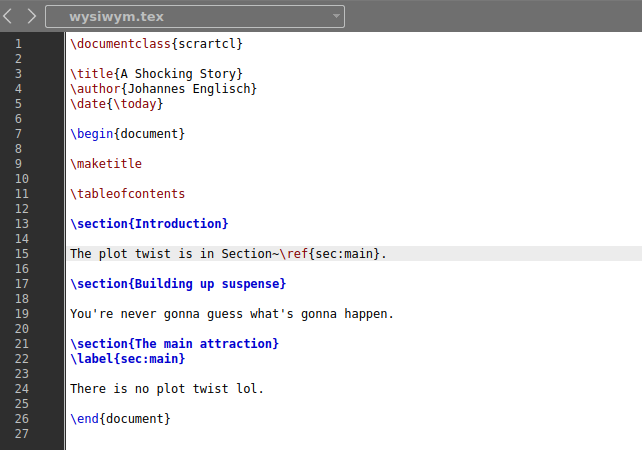
\includegraphics[width=0.8\textwidth]{images/code-snippet.png}
  \end{center}
\end{frame}

\begin{frame}
  \frametitle{What \emph{do} you see? (ctd.)}

  \begin{center}
    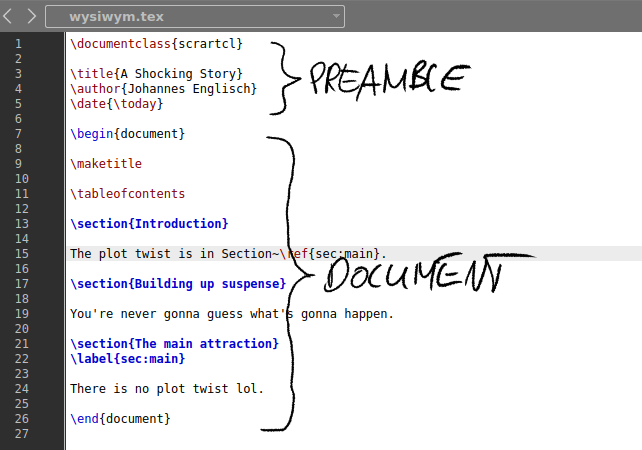
\includegraphics[width=0.8\textwidth]{images/preamble.png}
  \end{center}
\end{frame}

\begin{frame}
  \frametitle{What \emph{do} you see? (ctd.)}

  \begin{center}
    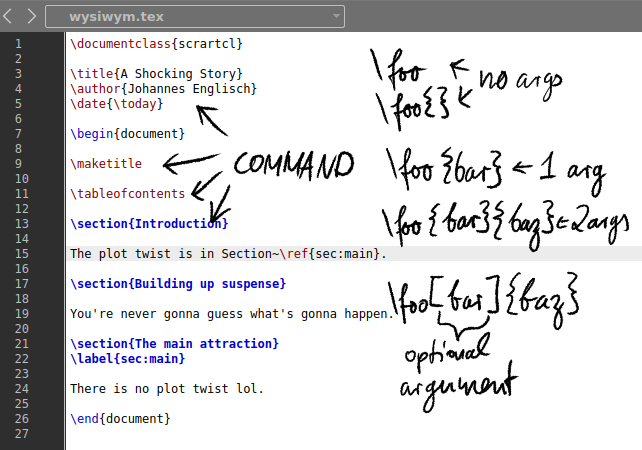
\includegraphics[width=0.8\textwidth]{images/command.png}
  \end{center}
\end{frame}

\begin{frame}
  \frametitle{What \emph{do} you see? (ctd.)}

  \begin{center}
    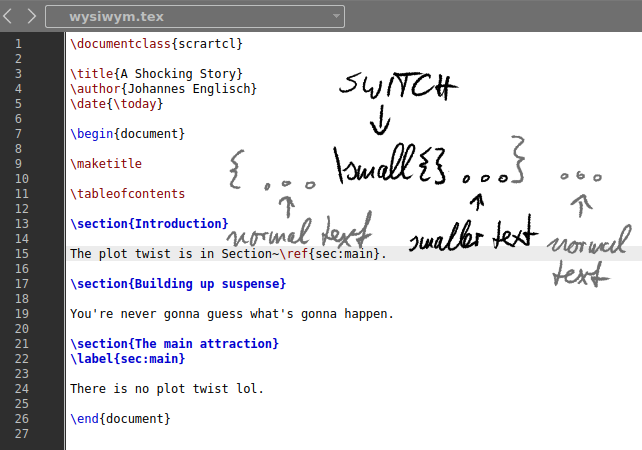
\includegraphics[width=0.8\textwidth]{images/switch.png}
  \end{center}
\end{frame}

\begin{frame}
  \frametitle{What \emph{do} you see? (ctd.)}

  \begin{center}
    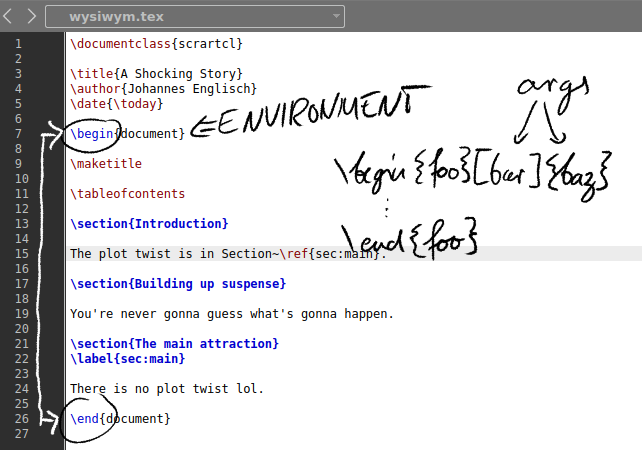
\includegraphics[width=0.8\textwidth]{images/environment.png}
  \end{center}
\end{frame}

\begin{frame}
  \frametitle{Let's get our hands dirty!}

  \begin{center}
    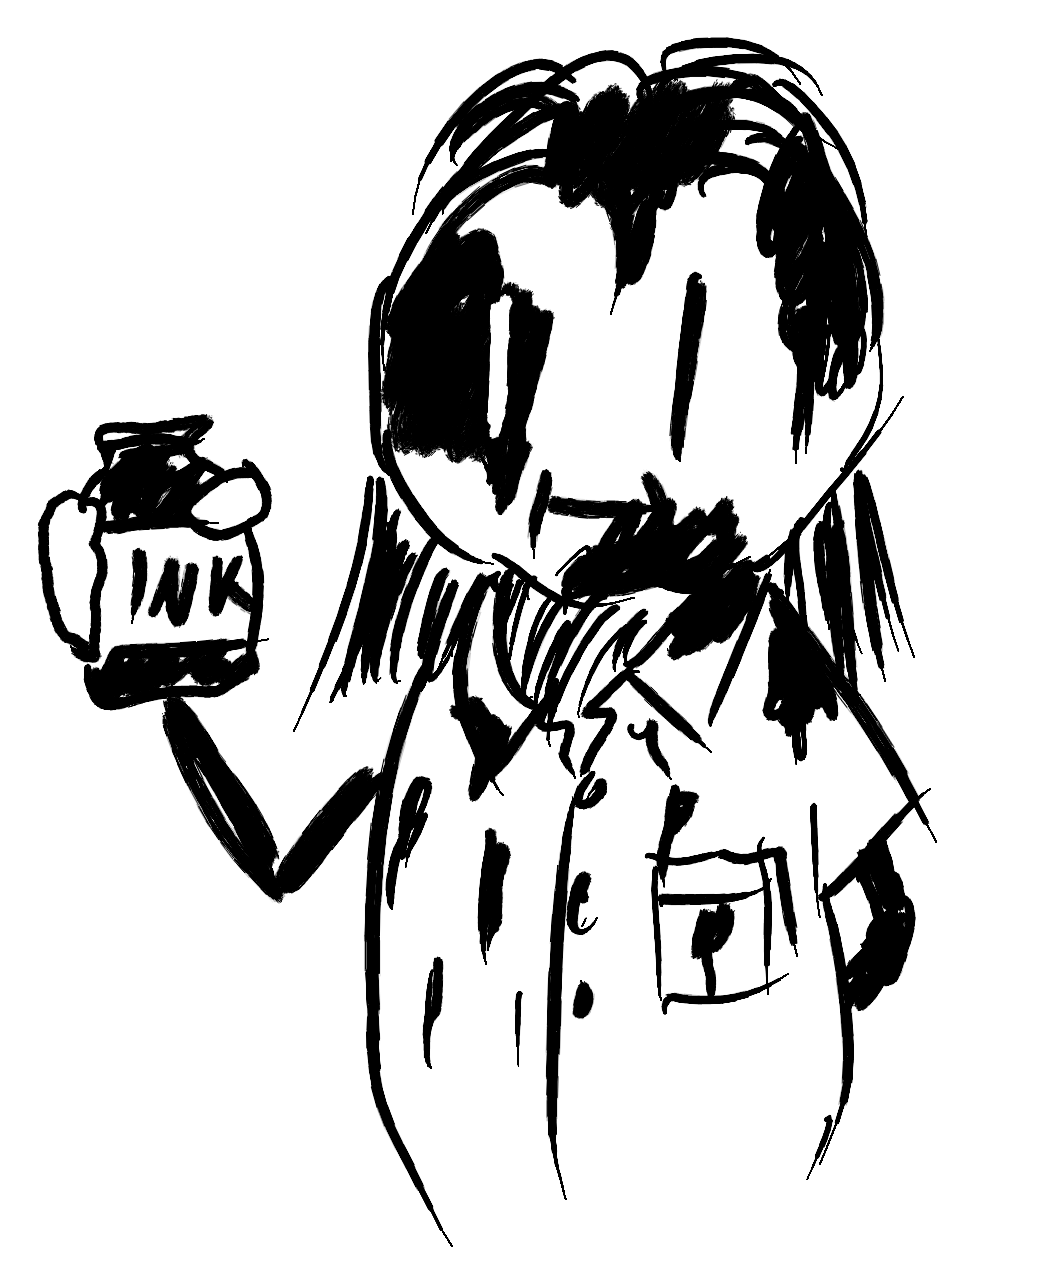
\includegraphics[width=0.5\textwidth]{images/dirty.png}
  \end{center}
\end{frame}

\section{The End}

\begin{frame}
  \frametitle{What now?}

  \begin{block}{Some links}
    \begin{itemize}
      \item The \LaTeX{} book on \href{https://en.wikibooks.org/wiki/LaTeX}{Wiki Books}.
      \item \dots{}which has a~\href{https://en.wikibooks.org/wiki/LaTeX/Linguistics}{chapter on linguistics}.
      \item \url{https://tex.stackexchange.com/}
      \item \href{https://detexify.kirelabs.org/classify.html}{Detexify}:
        If you don't know the \LaTeX{} command for a~special symbol, just draw
        it into the field.
      \item I~don't think Overleaf is a~good idea but
        \href{https://www.overleaf.com/learn}{their documentation section}
        is pretty rad.
      \item These slides:\\
        {\small\url{https://github.com/johenglisch/latex-intro-2023-10}}
    \end{itemize}
  \end{block}
\end{frame}

\end{document}
